\section{Servidor na nuvem}

O servidor na nuvem tem a responsabilidade de realizar a comunicação entre as aplicações cliente disponíveis para o usuário final e as casas inteligentes, de armazenar os dados coletados pelos sensores e de realizar processamentos que sejam muito onerosos para a capacidade de processamento dos dispositivos físicos. A seguir, são explorados os conceitos que orientaram o design da arquitetura e a implementação do servidor do Hedwig.

\subsection{Computação em nuvem}

O projeto Hedwig opta por uma solução voltada à nuvem. Os componentes do servidor são hospedados na nuvem pelas seguintes vantagens \cite{viswanathan}:

\begin{itemize}
\item \textbf{Custo} - o investimento em servidores próprios geralmente possui um alto custo. Em contrapartida, os fornecedores de \emph{Infrastructure as a Service} oferecem várias modalidades de precificação que vão desde assinaturas periódicas até pacotes que impõem limites de requisições.
\item \textbf{Escalabilidade} - existe uma grande facilidade em escalar os recursos de forma rápida. Os serviços de nuvem permitem manipular características como capacidade de disco, tamanho de memória e tipo de processador das instâncias que rodam os programas e aplicações. Também é possível seguir o caminho da escalabilidade horizontal e simplesmente replicar instâncias ao invés de melhorar suas especificações técnicas.
\item \textbf{Alocação de recursos eficiente} - com a precificação flexível e a facilidade em escalar, é possível aproveitar melhor a capacidade de processamento disponível e evitar desperdício com recursos ociosos.
\item \textbf{Backup e recuperação de dados} - os serviços de nuvem já providenciam funcionalidades de backup e restauração de dados, que podem ser tarefas arduosas para realizar em dispositivos físicos.
\end{itemize}

\subsection{Banco de dados não-relacional}

Bancos de dados não-relacionais são modelados em forma alternativa às tabelas relacionais dos sistemas SQL. São muitas vezes chamados de bancos NoSQL, que adquiriu o significado de \emph{Not Only SQL} \cite{nosql}. Algumas das características predominantes são a facilidade de escalabilidade horizontal, por meio de replicação e “clusterização”, e a priorização da disponibilidade ao invés da consistência. Esse último ponto pode ser sintetizado no conceito de BASE - \emph{Basically Available, Soft state, Eventual consistency} -, que é colocado em contraposição às garantias popularmente oferecidas pelos bancos relacionais: Atomicidade, Consistência, Isolamento, Durabilidade (\emph{Atomicity, Consistency, Isolation, Durability} - ACID). Apesar disso, alguns dos bancos NoSQL possuem características compatíveis com ACID. Esse tipo de banco de dados é bastante utilizado em aplicações web de tempo real e de Big Data \cite{pereira}.

Os bancos de dados NoSQL podem usar vários esquemas para modelar os dados que armazenam: colunas, documentos, pares chave-valor, grafos ou uma mistura dos anteriores. Dentre eles, destacam-se os documentos, também chamados de dados semi-estruturados. Documentos são dados codificados em XML, JSON, YAML ou em outros formatos ou códigos, incluindo até mesmo binários. Geralmente, não seguem nenhum esquema rígido, o que torna o desenvolvimento mais flexível e facilita a incrementação dos modelos com novos dados.

\subsection{Banco de dados em memória}

Bancos de dados em memória usam a memória principal do computador para realizar o armazenamento de dados ao invés de dispositivos de armazenamento em disco \cite{raima}. Como o tempo de acesso em disco é muito maior, esse tipo de banco de dados é capaz de atingir altos níveis de performance, proporcionando latências menores e mais previsíveis.

É um método de armazenamento mais caro \cite{mullins}, visto que a unidade de espaço em RAM é mais cara a de que disco. Assim, muitos projetos optam por uma arquitetura híbrida que usa tanto esse tipo de banco de dados quanto os tradicionais de acesso em disco. Devido ao fato da memória RAM ser volátil, esse tipo de abordagem também é usado para evitar perdas de dados em casos de falhas.

\subsection{WebSockets}

WebSocket é um protocolo de comunicação \emph{full-duplex} sobre conexões TCP. Ele possibilita a comunicação interativa entre cliente e servidor sem a necessidade de disparar múltiplas requisições HTTP, permitindo também que o servidor envie conteúdo ao cliente sem que este tenha que requisitá-lo.

É um protocolo da camada de aplicação compatível com HTTP: a transição entre esses dois protocolos é feita por meio de um handshake que usa o cabeçalho de HTTP Upgrade, como observado na figura a seguir.

A sua arquitetura diminui as latências de comunicação, fazendo-o ser um protocolo popular entre aplicações de tempo real. A compatibilidade com HTTP permite que toda a troca de dados ocorra nas portas 80 ou 443, mitigando os problemas de incompatibilidade com ambientes que possuem firewalls bloqueando certas portas TCP. A maioria dos navegadores modernos implementa o protocolo de WebSockets, possibilitando o funcionamento de aplicações de chat e de notificações.

\subsection{WebSockets}

WebSocket é um protocolo de comunicação full-duplex sobre conexões TCP \cite{rfc6455}. Ele possibilita a comunicação interativa entre cliente e servidor sem a necessidade de disparar múltiplas requisições HTTP, permitindo também que o servidor envie conteúdo ao cliente sem que este tenha que requisitá-lo.

\begin{figure}[H]
	\centering
	\caption{Comparação entre WebSockets e \emph{polling}}
  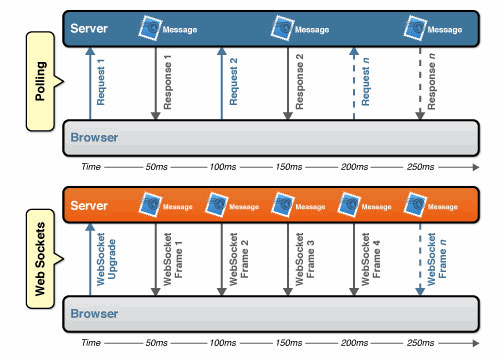
\includegraphics[width=0.7\textwidth]{websocketVsPolling}
	\caption*{Fonte: \cite{lubbers}}
\label{fig:websocketVsPolling}
\end{figure}

É um protocolo da camada de aplicação compatível com HTTP: a transição entre esses dois protocolos é feita por meio de um handshake que usa o cabeçalho de HTTP Upgrade, como observado na figura a seguir.

A sua arquitetura diminui as latências de comunicação, fazendo-o ser um protocolo popular entre aplicações de tempo real. A compatibilidade com HTTP permite que toda a troca de dados ocorra nas portas 80 ou 443, mitigando os problemas de incompatibilidade com ambientes que possuem firewalls bloqueando certas portas TCP. A maioria dos navegadores modernos implementa o protocolo de WebSockets, possibilitando o funcionamento de aplicações de chat e de notificações.

\subsection{Arquitetura de Microsserviços}

\subsubsection{Características}
A arquitetura de microsserviços é um estilo que compreende a estruturação de uma aplicação em um conjunto de serviços com baixo grau de acoplamento que se comunicam por meio de protocolos de comunicação leves.

Para melhor compreender essa arquitetura, podemos compará-la à arquitetura monolítica. Uma aplicação monolítica está contida em uma única unidade, que geralmente é dividida em camadas de funcionalidade tecnológica como interface web, camada de negócios server-side e camada de persistência de dados. A escalabilidade desse modelo é dada por meio do aumento do número de servidores, máquinas virtuais ou contêineres juntamente a um load balancer - é a chamada escalabilidade horizontal. Uma alteração em uma pequena parte da aplicação significa que toda a aplicação deverá passar por um processo de \textit{build} e \textit{deploy}. Já a arquitetura de microsserviços divide as funcionalidades em serviços autônomos, muitas vezes usando as regras de negócios para realizar essa divisão. Cada serviço tem seu próprio ciclo de desenvolvimento e pode ser atualizado independentemente. A escalabilidade também é tratada serviço a serviço.

\begin{figure}[H]
	\centering
	\caption{Comparação entre uma aplicação monolítica (esquerda) e com microsserviços (direita)}
  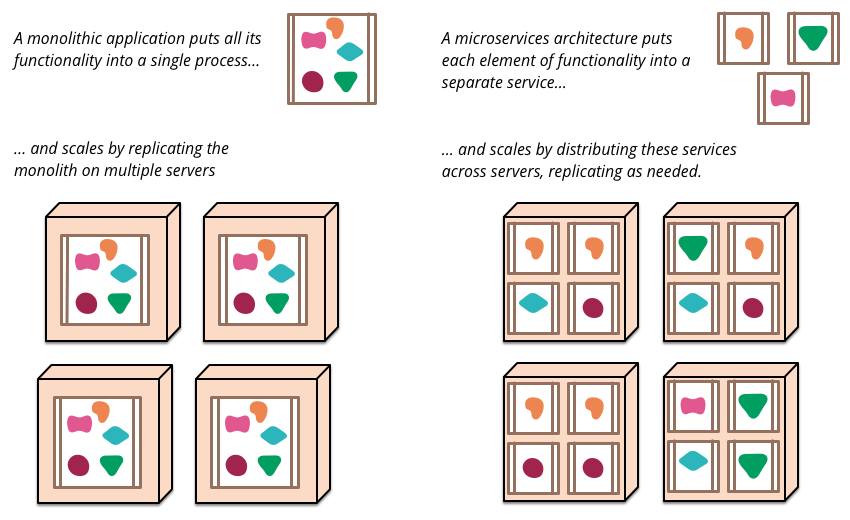
\includegraphics[width=0.8\textwidth]{estruturaMicrosservicos}
	\caption*{Fonte: \cite{lewis}}
\label{fig:estruturaMicrosservicos}
\end{figure}

É difícil delimitar uma definição formal para arquitetura de microsserviços, pois não existe consenso a respeito de sua definição formal. Contudo, existe uma série de características que projetos usando essa arquitetura compartilham. Detalhamos a seguir alguns atributos e aspectos dos microsserviços. Nem todos os projetos possuem rigorosamente todas as características, mas a maioria deles possui um perfil similar ao descrito aqui.

\begin{itemize}
\item \textbf{Serviços são processos.}Pode-se fazer um mapeamento de um processo para um serviço, porém isso é apenas uma aproximação, podendo um serviço ser constituído por uma aplicação de múltiplos processos.
\item \textbf{Serviços comunicam-se por protocolos leves.}Geralmente, são usados protocolos como o HTTP.
\item \textbf{Serviços implementam capabilidades do negócio.}Isto é, a divisão de serviços é baseada nas regras de negócio e nas funcionalidades que o produto deverá suprir.
\item \textbf{Serviços são facilmente substituíveis.}
\item \textbf{Cada serviço tem um ciclo de vida independente.}Isso inclui o desenvolvimento e os processos de \textit{deploy}. Um microsserviço pode ser implementado e atualizado independentemente dos outros.
\end{itemize}

As vantagens da arquitetura de microsserviços giram em torno da modularidade e autonomia dos serviços que é natural à sua estrutura. Com isso, pode-se ter uma heterogeneidade de tecnologias, isto é, cada serviço pode ser desenvolvido usando diferentes linguagens, \textit{frameworks} e ferramentas de acordo com seus requisitos. A independência entre serviços também possibilita o deploy automatizado e o uso de práticas de integração contínua. Também há benefícios de aspecto gerencial: como cada serviço tem como escopo uma capabilidade do negócio que envolve interfaces de interação com usuário, código em várias camadas que implementa as funcionalidades necessárias e persistência em bancos de dados, é possível criar pequenas equipes multidisciplinares para cada microsserviço.

Existem trade-offs que devem ser considerados ao decidir pela arquitetura de microsserviços. A comunicação entre serviços por meio de uma rede possui maior latência e exige maior processamento do que mensagens trocadas a nível de processos. Por isso, é muito importante analisar as fronteiras dos serviços e a alocação de responsabilidades durante do projeto. A descentralização de dados entre microsserviços traz também a necessidade de métodos para manter a consistência das informações. Outro ponto crítico são sistemas com alta granularidade de microsserviços, causando overhead tanto de comunicação como de código além de uma fragmentação lógica que causa mais impactos negativos na complexidade e performance do que benefícios - tal caso de antipadrão foi chamado de nanosserviço \cite{rotem}.

% TODO melhorar paragrafo abaixo
Os microsserviços podem ser vistos como um estilo específico de arquitetura orientada a serviços (\textit{Service-oriented architecture} - SOA), visto que existem várias características compartilhadas entre os dois. Contudo, o termo arquitetura orientada a serviços é muito amplo, e muitas de suas implementações podem não seguir certos pontos apresentados como aspectos dos microsserviços, como por exemplo, o uso de grande inteligência no mecanismo de comunicação de dados ao invés de delegar tal complexidade aos endpoints do serviço \cite{james}. Esse e outros problemas conhecidos das experiências passadas de sistemas estruturados em SOA fazem com que muitos encarem os microsserviços como uma modernização da arquitetura orientada a serviços.

Apesar do termo microsserviço ter surgido por volta de 2011 \cite{james}, as ideias por trás desse estilo arquitetural não são recentes. O aumento da discussão em torno dos microsserviços nos últimos anos pode ser creditada a avanços tecnológicos tais como a disseminação dos serviços de nuvem, o crescimento de ferramentas de automatização de implantação, a consolidação dos conceitos de DevOps, entre outros.
